%************************************************
\chapter{Introducción}\label{ch:introduction}
%************************************************

En la actualidad, para demostrar que conocemos un secreto a alguien, utilizamos un medio donde nadie nos espíe y le contamos el secreto directamente a nuestro interlocutor. En el ámbito de la criptografía, cifraríamos el secreto con una clave, simétrica o asimétrica, tal que, sólo quien conozca la clave de descifrado pueda leer nuestro secreto. Esto es la base de las comunicaciones seguras en Internet. Ciframos nuestra contraseña de modo que sólo el servidor de correo pueda leerla, pudiendo iniciar nuestra sesión sin que ningún espía nos la pueda robar. El problema es que hay dos partes que conocen el secreto, dos puntos de ataque.

Existe un área de la criptología que se encarga de abordar este problema, demostrar que conocemos algo, pero sin que de la misma prueba se obtenga más información. Estos métodos se conocen como Pruebas de Conocimiento Cero. Para ilustrar estas pruebas, en 1990 Guillou, Quisquater y Berson publicaron en \textit{How to Explain Zero-Knowledge Protocols to Your Children} \citep{ZKPcave:story} una historia sobre cómo Alí Babá demostró poder abrir la cueva sin decir a nadie cuáles eran las palabras mágicas. Aquí presentamos una versión resumida que destaca las propiedades básicas de estos métodos:

\hfil

\begin{quote}
Imaginemos una cueva, donde el camino principal se bifurca y al final de cada pasillo los caminos se vuelven a encontrar, formando una especie de anillo. En el punto en que se unen, dentro de la cueva, hay una puerta mágica con una palabra secreta, la cual permite abrirla y cruzar al otro lado.

\textbf{P}aula conoce la clave secreta y quiere \textbf{p}robarlo a su amigo Víctor, pero sin tener que revelársela.
\marginpar{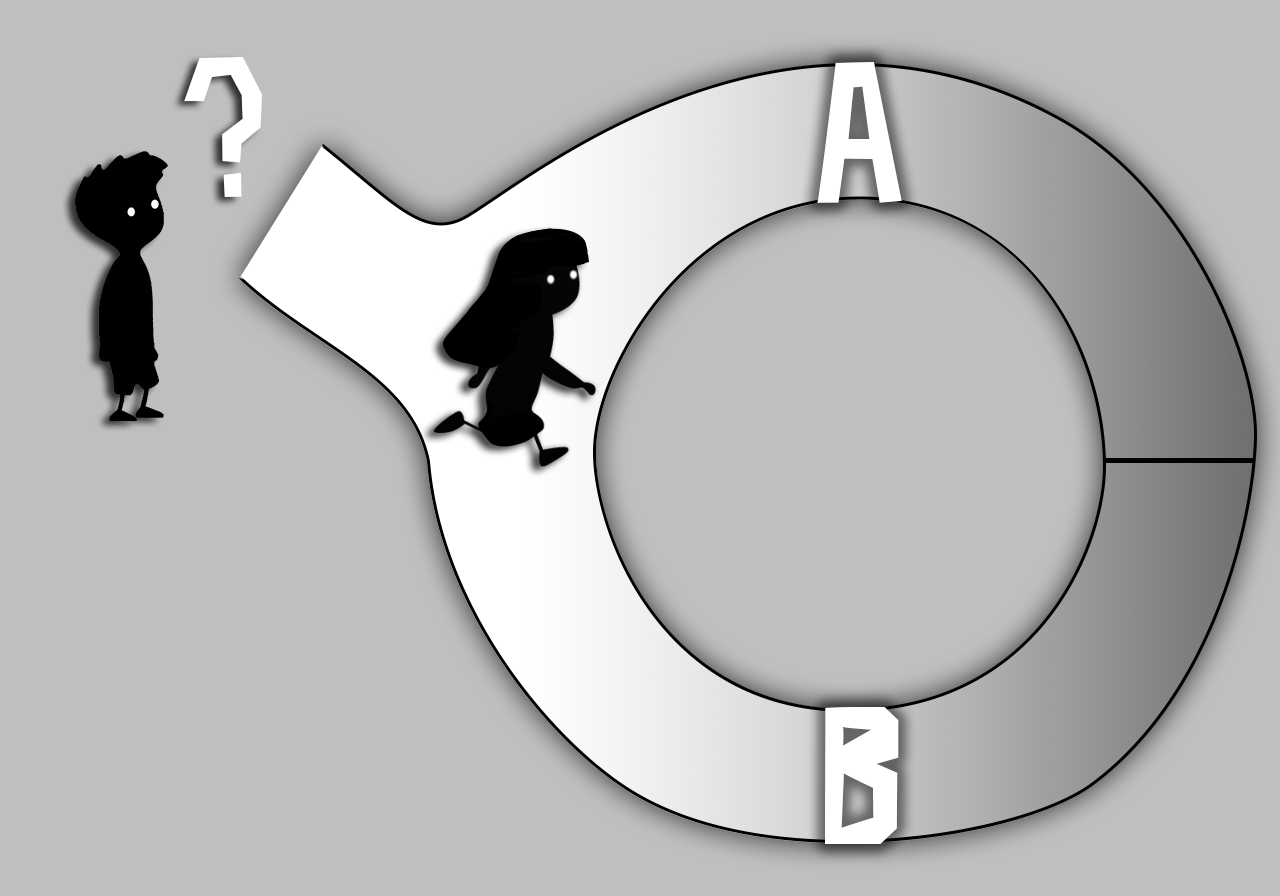
\includegraphics[width=1.\linewidth]{gfx/graficoJL_ZKP_1}\\La cueva \citep{ZKPcave:fig}
. Paula entra por A o B al azar. Víctor espera fuera.}
Paula y Víctor quedan en la entrada de la cueva con unos \textit{walkie-talkies}, de modo que Víctor esperará fuera y Paula entrará a la cueva y tomará uno de los pasillos, que llamaremos A y B, sin decirle cuál a Víctor.

%\begin{figure}[bth]
%	\begin{center}
%		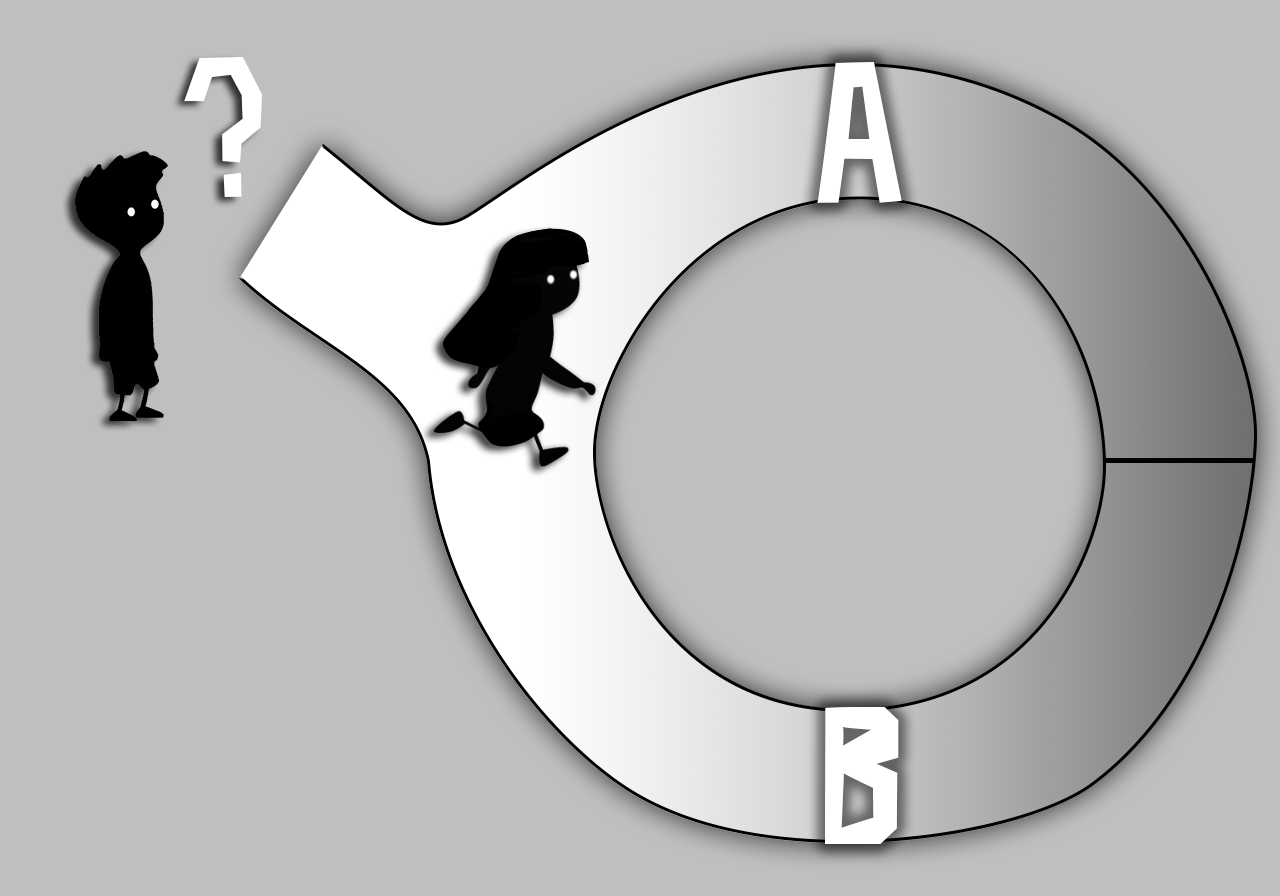
\includegraphics[width=.45\linewidth]{gfx/graficoJL_ZKP_1}
%	\end{center}
%	\caption{La cueva \citep{ZKPcave:fig}. Paula entra por A o B al azar, Víctor espera fuera.}
%	\label{fig:ZKPcave1}
%\end{figure}

Al llegar a la puerta, Paula avisa a Víctor para que entre a la cueva y espere en la bifurcación, donde \textbf{V}íctor, para intentar \textbf{v}erificar que Paula conoce la palabra secreta, le indicará por qué pasillo quiere que vuelva, el A o el B.


%\begin{figure}[bth]
%	\begin{center}
%		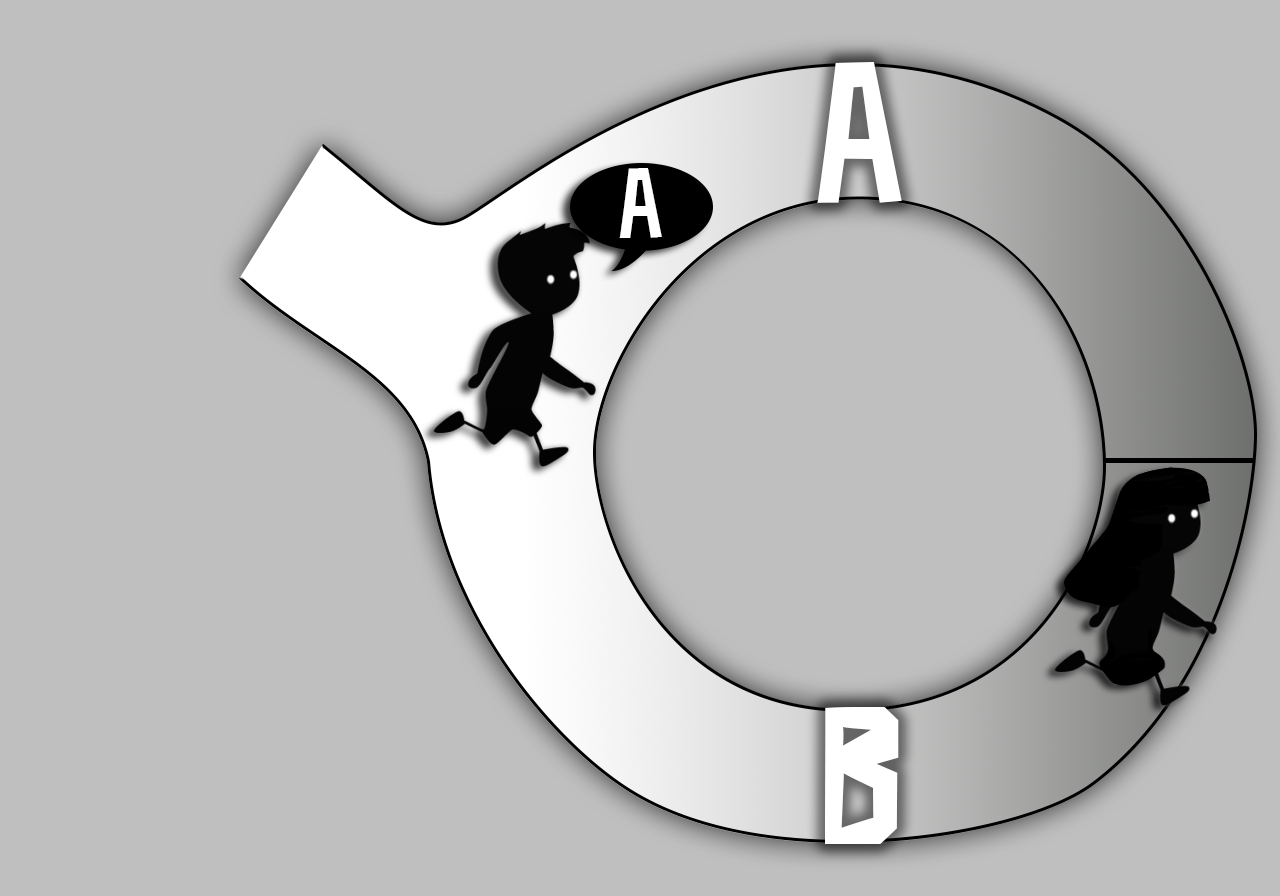
\includegraphics[width=.45\linewidth]{gfx/graficoJL_ZKP_2}
%	\end{center}
%	\caption{La cueva. Víctor elige al azar por dónde quiere que regrese Paula.}
%	\label{fig:ZKPcave2}
%\end{figure}

Si Paula realmente conoce el secreto, podrá volver a la bifurcación por el pasillo solicitado, abriendo, si es preciso, la puerta.\marginpar{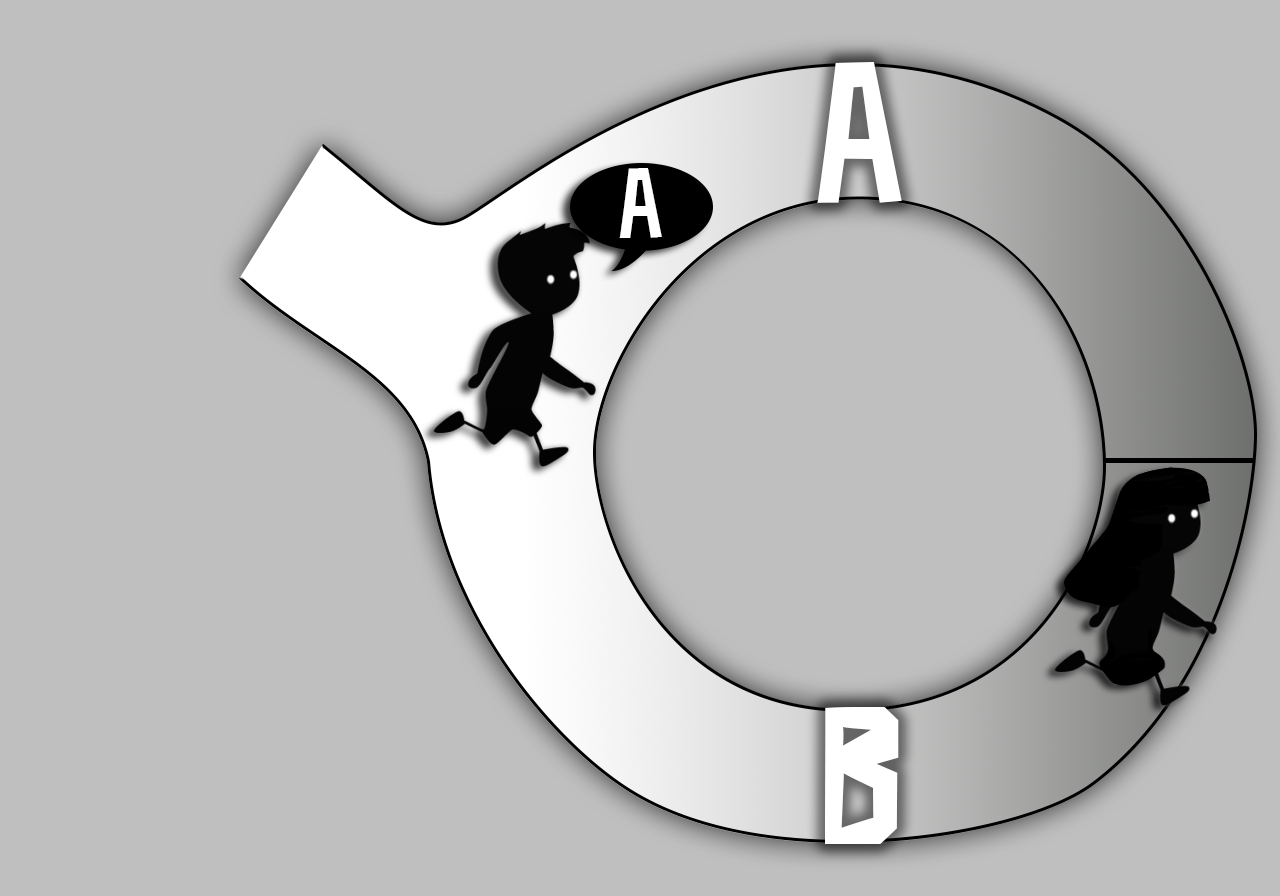
\includegraphics[width=1.\linewidth]{gfx/graficoJL_ZKP_2}\\La cueva. Víctor elige al azar por dónde quiere que regrese Paula.}
Pero en caso de no conocer la clave, al entrar por uno de los pasillos, tenía una probabilidad del $50\%$ de adivinar cuál pediría Víctor.


%\begin{figure}[bth]
%	\begin{center}
%		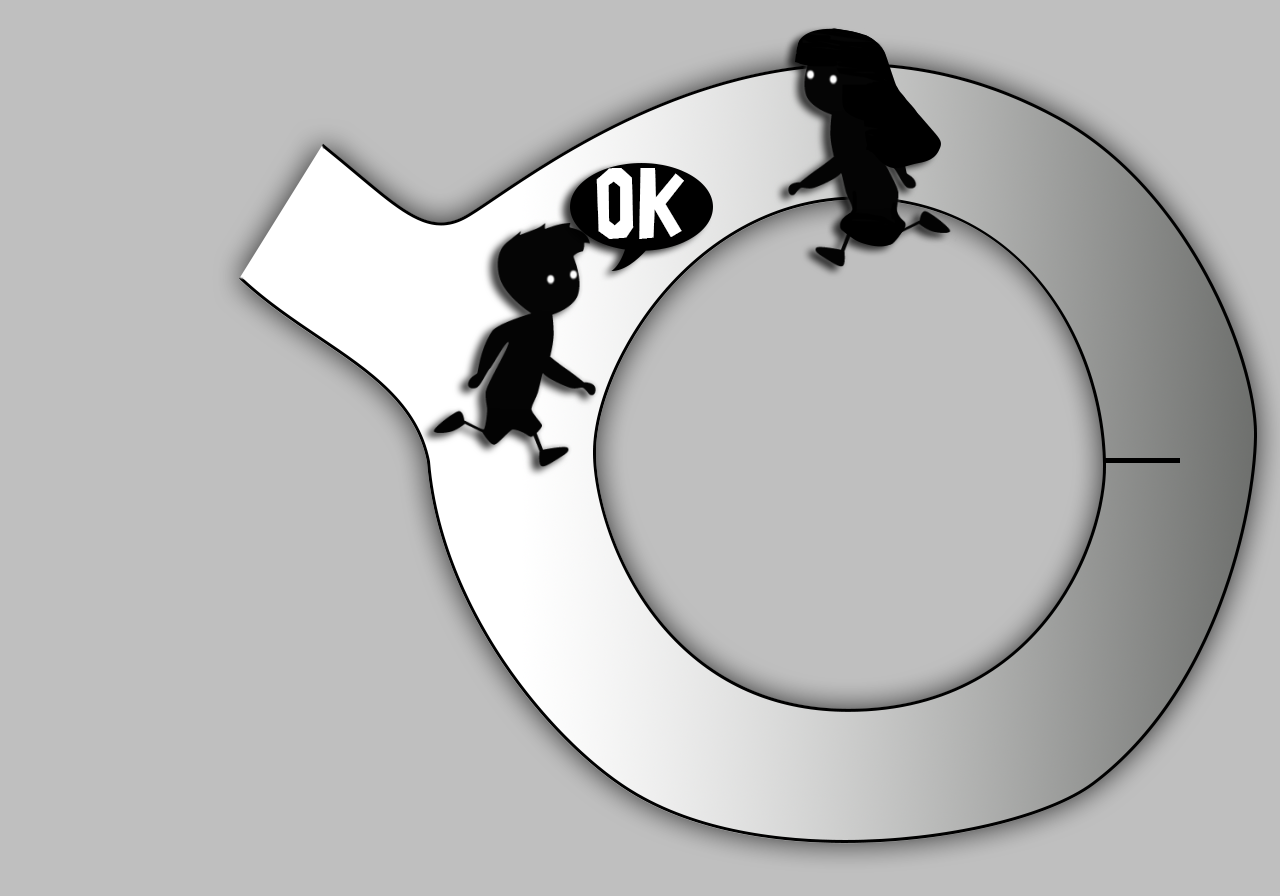
\includegraphics[width=.45\linewidth]{gfx/graficoJL_ZKP_3}
%	\end{center}
%	\caption{La cueva. Paula vuelve por el camino pedido.}
%	\label{fig:ZKPcave3}
%\end{figure}

Víctor no se queda contento con una sola prueba, pues Paula podría haber tenido suerte, así que la repiten hasta que se convence. Con unas 20 repeticiones, Paula tendría solo una probabilidad de $2^{-20}$, prácticamente nula, de acertar todas las veces y engañar así a Víctor.
\marginpar{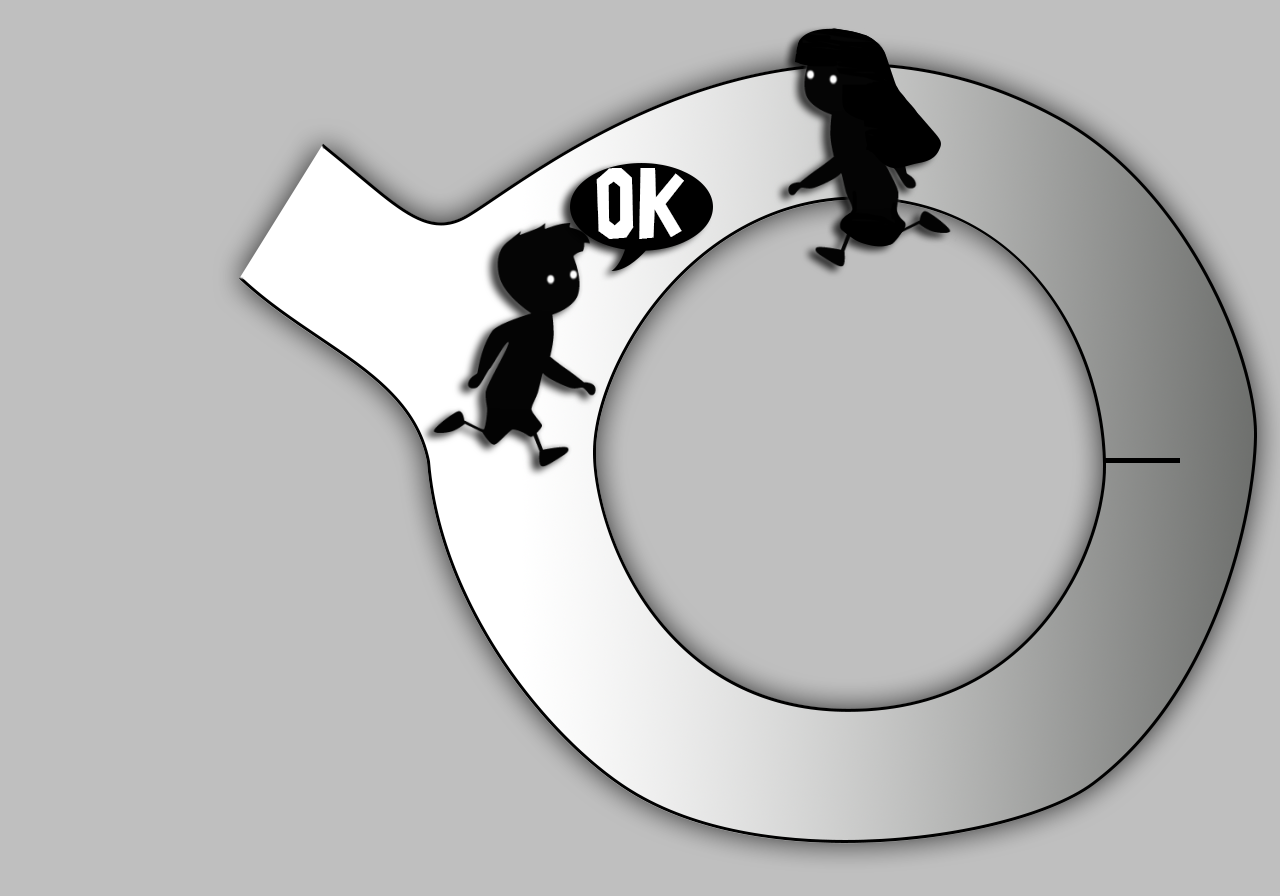
\includegraphics[width=1.\linewidth]{gfx/graficoJL_ZKP_3}\\La cueva. Paula vuelve por el camino pedido.}


\textbf{E}va, curiosa de qué hacían Víctor y Paula en la cueva, \textbf{e}spía a Víctor durante todo el proceso. Eva no sabe si Paula y Víctor han acordado previamente qué pasillo pedir por el \textit{walkie-talkie}, y sólo Víctor está seguro de que él los estaba eligiendo al azar y sin previo acuerdo.%, por eso, Eva no puede estar segura de si Paula conoce la clave secreta, o bien estaban \textbf{s}imulando todo para engañarla por cotilla.

Más tarde Eva habla con Víctor, que está seguro de que Paula conoce la clave, y éste querría convencer también a Eva, pero como él no conoce la clave, no puede repetir la prueba a Eva, sólo Paula puede realizarla con éxito.
\end{quote}


\hfil

En el estudio formal de las Pruebas de Conocimiento Cero se utilizan distintos tipos de problemas, y los más utilizados pertenecen a las áreas de \textbf{álgebra} y \textbf{grafos}. Son problemas difíciles de resolver para quien no conoce alguna información extra de los mismos, que en nuestra fábula serían el problema de abrir la puerta sin conocer la palabra mágica. Los problemas más representativos de las Pruebas de Conocimiento Cero son el del logaritmo discreto, la raíz cuadrada modular o residuos cuadráticos, el isomorfismo de grafos y la 3-coloración de grafos.

Primero deberemos definir qué se entiende por un problema \textit{difícil}, para ello, en el capítulo TODO, se introducirán unos preliminares de computación, que estudian y clasifican los problemas. A continuación, estudiaremos la teoría relacionada con cada problema \textit{difícil} utilizado en las Pruebas de Conocimiento Cero que vamos a ver: en el capítulo TODO, veremos el álgebra relacionada con el logaritmo discreto, en el capítulo TODO, las definiciones y teoremas necesarios para conocer los residuos cuadráticos, y en el capítulo TODO la teoría básica de grafos necesaria para comprender los problemas.

Una vez conocemos la teoría detrás de cada problema, podremos estudiar, en el capítulo TODO, las Pruebas de Conocimiento Cero, definiremos qué propiedades debe cumplir una prueba de este tipo, enunciaremos pruebas que utilicen los problemas anteriores, y demostraremos que cada una de ellas cumple la definición. Finalmente, daremos algunas aplicaciones prácticas equivalentes a las de la criptografía actual en el capítulo TODO.


